% el problema
El problema del \textit{trafico} que consideraremos tiene la siguiente premisa. Dado una ciudad representada por $n$ puntos conectados por $m$ calles unidireccionales, dos puntos críticos $s$ y $t$, y un conjunto
\begin{equation*}
    P := \{p_1 \ ... \ p_k\}    
\end{equation*}
de $k$ calles bidireccionales candidatas, queremos saber por cuánto podemos mejorar la distancia mínima entre $s$ y $t$, de construir una de estas calles.

Para ello, vamos a contar con la longitud $l_i$, $1 \leq i \leq n$ de cada calle en la ciudad y la longitud $l_j$, $1 \leq j \leq k$ de cada calle candidata.

Por ejemplo, si tuvieramos la siguiente ciudad, puntos críticos $s = 1$ y $t = 4$ y las calles candidatas marcadas en gris
\begin{figure}[!htbp]
    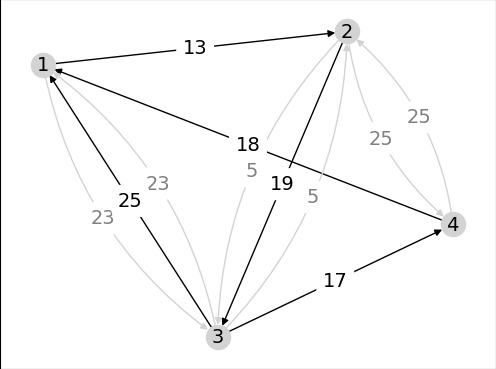
\includegraphics[scale=0.6, trim={0.2cm 0.2cm 0.2cm 0.2cm}, clip]{/files/src/.media/grafo.png} 
    %\caption{s} \label{ejemplo}
\end{figure}
    
\noindent podríamos construir la calle $2 \leftrightarrow 3$ con peso $5$ para lograr una distancia mínima de largo $35$.

% modelado
\subsection{Modelado como un problema de camino mínimo}\label{modelo}

% optimalidad
\subsection{Demostración de optimalidad}

% correctitud
\subsection{Demostración de correctitud}\label{correctitud} 

% algoritmo
\subsection{El algoritmo} 

% complejidad
\subsection{Complejidad temporal y espacial} 
